\section{Where the queue forms}
\label{sec:results}

\begin{figure}[t]
\centering
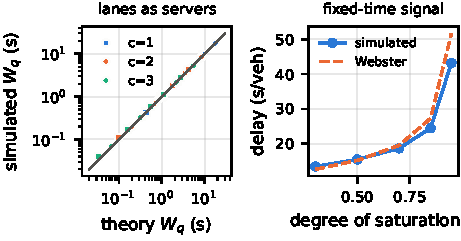
\includegraphics[width=\columnwidth]{figures/validation.pdf}
\caption{Validation. Left: simulated versus theoretical mean wait for
1--3 servers (lanes), Poisson arrivals, exponential (circles) and
deterministic (squares) service, $\rho = 0.3$--$0.9$. Right: delay at a
fixed-time signal (90\,s cycle, $g/C = 0.5$) versus Webster.}
\label{fig:validation}
\end{figure}

\paragraph{Validation.} The discrete-event simulator matches Erlang C,
M/D/1 and Allen--Cunneen with a mean error of \ValErr\% over \ValN\
settings (worst \ValErrMax\%, Allen--Cunneen at light load), and
Webster's signal delay within \ValSigErr\% on average
(Figure~\ref{fig:validation}). Without capacity drop, the CTM's total
delay behind a single lane drop equals the fluid point queue to within
\ValCtmFluidErr\%, as Newell's equivalence requires
\cite{newell1993kinematic}.

\paragraph{The lane count overstates demand by an order of magnitude.}
If every feeder lane discharged at saturation, the \AnaEBSideLanes\
eastbound feeder lanes would deliver about \AnaEBSatVph\,veh/h. Under the
base rates they deliver \AnaEBSideVph\,veh/h, or \AnaEBPerLane\,veh/h per
lane (\AnaEBPerLanePct\% of saturation; westbound \AnaWBPerLane\,veh/h,
\AnaWBPerLanePct\%). Half the approaches are driveways and most of the
rest are one-lane residential streets. Because exits balance the side
inflow, peak corridor flow reaches only \AnaEBPeakFlow\,veh/h eastbound
and \AnaWBPeakFlow\,veh/h westbound.

\begin{figure}[t]
\centering
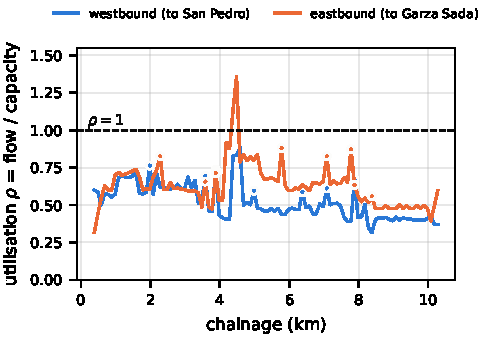
\includegraphics[width=\columnwidth]{figures/utilisation.pdf}
\caption{Steady-state utilisation along the corridor at base parameters;
dots mark signalised cells. Both directions exceed $\rho = 1$ only at the
five-to-three-lane merge near 4.5\,km.}
\label{fig:rho}
\end{figure}

\paragraph{Utilisation picks one place.} Figure~\ref{fig:rho} shows $\rho$
along both directions. It stays below one everywhere except at the merge
between the Alfonso Reyes overpass and the Arroyo Seco bridge, where it
reaches \AnaEBMaxRho\ eastbound. Westbound it peaks at \AnaWBMaxRho\
at the same place. It would be \NcWBMaxRho\ with the assumed demand at
Alfonso Reyes instead of the field estimate. Signals raise $\rho$ locally
but do not push it over one at base parameters.

\begin{figure*}[t]
\centering
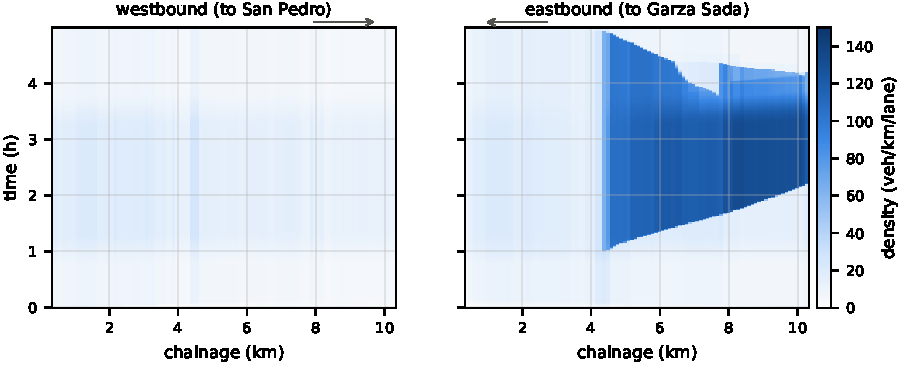
\includegraphics[width=\textwidth]{figures/spacetime.pdf}
\caption{CTM density over time and space at base parameters, both drawn
with chainage increasing to the right (arrows give the travel direction).
Eastbound the queue head stays at the merge (\PeakEBHeadKm\,km) and
backs up across the whole upstream corridor to Gómez Mor\'in; westbound,
with the Alfonso Reyes field estimate, no queue forms.}
\label{fig:spacetime}
\end{figure*}

\paragraph{The peak.} In the CTM (Figure~\ref{fig:spacetime}) the
westbound direction stays free-flowing at base demand. With the assumed
demand at Alfonso Reyes it would queue for \NcWBQueueKm\,km and lose
\NcWBDelay\,veh\,h, so one roadside estimate is enough to remove a
predicted queue. The eastbound queue forms at \PeakEBHeadKm\,km, fills the
\PeakEBQueueKm\,km upstream to Gómez Mor\'in and costs
\PeakEBDelay\,veh\,h (\PeakEBPerVeh\ min per vehicle). A single-bottleneck
fluid queue at the merge would predict \PeakEBFluid\,veh\,h. The
difference comes from the queue reaching feeders and exits upstream. That
is the most uncertain part of the model: with exits that leave freely
($\phi = 0$) eastbound delay is \PeakEBFifoLo\,veh\,h, and with strict
FIFO it is \PeakEBFifoHi. The location of the head does not move.

\begin{figure}[t]
\centering
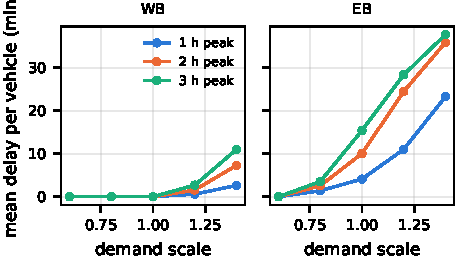
\includegraphics[width=\columnwidth]{figures/demand_grid.pdf}
\caption{Mean delay per vehicle versus a uniform demand scale, for peaks
of 1--3 hours.}
\label{fig:grid}
\end{figure}

\paragraph{Sensitivity to demand.} Scaling all demand
(Figure~\ref{fig:grid}), congestion appears at \GridEBOnset$\times$ base
eastbound and \GridWBOnset$\times$ westbound, where the merge
has about 10\% spare capacity. At
\GridEBTopScale$\times$ with a two-hour peak, mean delay reaches
\GridEBTopPerVeh\ minutes per vehicle eastbound. Delay grows faster than
linearly with peak length, as the fluid model predicts for a queue that
grows throughout the peak.

\begin{figure}[t]
\centering
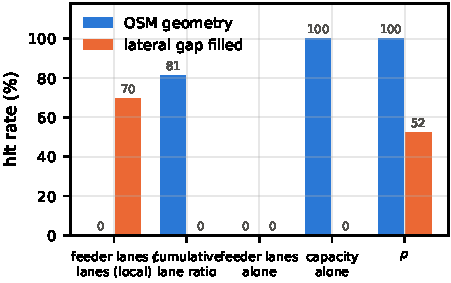
\includegraphics[width=\columnwidth]{figures/predictors.pdf}
\caption{How often each predictor's top segment is the CTM's principal
bottleneck, over \McDraws\ Monte Carlo draws $\times$ 2 directions
(congested runs only), with the OSM geometry and with the frontage gap
filled.}
\label{fig:predictors}
\end{figure}

\paragraph{The test.} Over \McDraws\ Monte Carlo draws of every
assumption (class rates, turn fractions, through demand, green ratio,
friction, $\phi$ and capacity drop), \McCongested\ of \McRuns\
direction-runs congest (Figure~\ref{fig:predictors}). The local lane ratio
picks the right segment in \McHitLR\% of them, and feeder lanes alone in
\McHitFC\%: the segments with the most feeders are not where the queue
starts. The cumulative lane ratio reaches \McHitLRC\%, but only through
its denominator, which drops at the merge. Utilisation reaches
\McHitRho\%. Its maximum also classifies congestion: $\max\rho \ge 1$
agrees with the CTM in \McAcc\% of runs (AUC \McAuc). The lane ratio
cannot do this at all, since it does not change with demand. The
hypothesis survives the falsification rule (falsified: \McFalsified).

There is a caveat, and the Monte Carlo makes it plain: capacity alone
also scores \McHitCap\%. With this geometry, the location is set by the
merge and demand only sets how bad it gets. To see what happens without
it, we fill the frontage gap and rerun. Then only \McGapCongested\ of
\McRuns\ runs congest, westbound congestion disappears at base parameters
($\max\rho = \GapWBMaxRho$; it does not congest at base parameters even with the gap), and eastbound the queue moves to
\GapEBHeadKm\,km. The location now depends on demand, and the ranking changes. Over the
\McGapCongested\ congested runs (all eastbound, mostly one segment), the
local lane ratio finds the bottleneck in \McGapHitLR\% of them,
utilisation in \McGapHitRho\% and capacity alone in \McGapHitCap\%.
Without the merge, the queue starts where many accesses join within a
short stretch. Friction and merge priority in the CTM pull the head there,
while steady-state $\rho$, which treats each cell on its own, points to a
neighbouring segment. So the lane-count argument is not wrong in general.
On this corridor, the lane drop decides the location, and the lane count
cannot see it.

\begin{figure}[t]
\centering
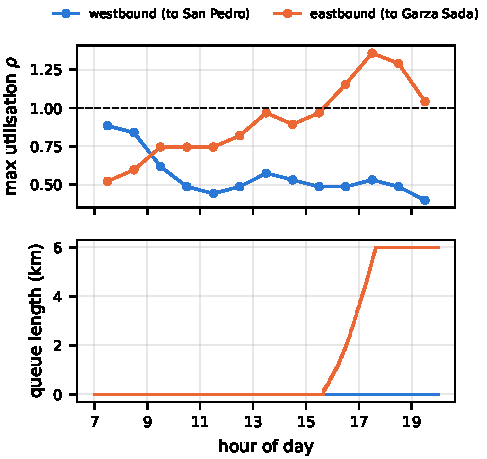
\includegraphics[width=\columnwidth]{figures/daily.pdf}
\caption{A working day, 7:00--20:00, with tidal demand (towards San Pedro
in the morning, towards Garza Sada in the evening). Top: maximum
utilisation along each direction, hour by hour. Bottom: queue length in
the CTM.}
\label{fig:daily}
\end{figure}

\paragraph{A working day.} The tests above use a generic two-hour peak.
Commuting is tidal. We assume that at 7:00 traffic heads south to north,
towards San Pedro and Valle Oriente, and that the evening reverses. The
hourly demand multipliers are set in the configuration
(Figure~\ref{fig:daily}). The maximum capacity at the merge is about
\DayWBCap\,veh/h westbound and \DayEBCap\,veh/h eastbound. With the
Alfonso Reyes estimates, westbound utilisation peaks at \DayWBMaxRho\ at
7:00 and no queue forms; across \DayDraws\ Monte Carlo days, a westbound
queue appears in \DayWBPQueue\%. Eastbound, $\rho$ passes one in the
afternoon. The queue forms at \DayEBStart, reaches \DayEBQueueKm\,km and
\DayEBClears: \DayEBCongH\ congested hours (median \DayEBCongHMed\ over
the Monte Carlo) and \DayEBDelay\,veh\,h within the window. The
observer reports little or no morning queue towards San Pedro, even
though the traffic from Carretera Nacional heads that way. That is the
one qualitative check we have against the field, and the model passes
it. The eastbound afternoon queue has no field check yet.
